\documentclass[12pt, titlepage]{article}
\usepackage[inner=1in,outer=1in,top=1in,bottom=1in]{geometry}
\usepackage[utf8]{inputenc}
\usepackage{fancyhdr}
\usepackage{amsmath}
\usepackage{amsfonts}
\usepackage{amssymb}
\usepackage{graphicx}
\usepackage{hyperref}
\usepackage{float}
\usepackage{listings}
\usepackage{multirow}
\setcounter{section}{0}
\pagestyle{fancy}

\lhead{STAT538 Final Report}
\rhead{Quanhan (Johnny) Xi}
\author{Quanhan (Johnny) Xi}
\title{STAT538 Final Report: Examining Socio-economic Factors of Secondary School Attendance via GLMs for Count Data}

\begin{document}
	\maketitle
	\section{Background and Objectives}
	\paragraph{} Secondary school absenteeism is an important indicator of a student's engagement in learning and their final outcomes. Chronic absenteeism has been shown to negatively impact students grades and standardized test scores where applicable. There is an existing literature that examines whether there may be systematic relationships between absenteeism and certain exogenous factors (\cite{Currie::2009}, \cite{Gubbels::2019}), which vary from the socio-economic and demographic states of the student, as well as the quality of curriculum and delivery. In this report, we will mainly focus on student-based factors, aiming to connect a student's personal situation with their absenteeism. Many of the variables that we examine can be viewed as degrees of distractions to a student's academics. Insights into which factors are truly affecting absenteeism, and to what degree, can help educators identify possible cases of high absenteeism earlier on in the academic year. For institutions, this can also provide insight into where resources should be allocated in order to improve student attendance and hence performance. 
	
	\paragraph{} Education is of great economic importance to regional and national governments. Early leaving of secondary education can be detrimental for a student's social development and cause extra strain on public services \cite{Rocque::2016}. We believe that regardless of government infrastructure, a person's lack of education is not typically determined by personal failure, but rather can be attributed to various, often uncontrollable factors in their early lives. By understanding some of these personal contributing factors to absenteeism, we aim to provide suggestions to tackle the root socio-economic causes of under-education. This provides an alternative perspective to this issue, in comparison to inadequacies in the education system alone. 
	
	\paragraph{} The data we consider is from Portugal, from the 2005-2006 academic year. According to the data authors, Portuguese students at this time had one of the highest dropout rates in the European Union (EU), at 40\% \cite{Cortez::2008}. Today, this has been reduced dramatically to 10 \%, but this remains one of the highest EU rates \cite{eurostat}. An interesting future study would be to repeat this analysis on the data today, and to examine whether absence rates, and the relationship between the corresponding indicators have changed. 
	
	\section{Dataset Description}
	\paragraph{} The data analyzed in this report is a concatenation of surveys from students in two Portuguese secondary schools. In total, there are 1044 observations over 30 measurements, of which we select 11 to include in our analysis. For each student, responses to a number of socio-economic queries and some demographic information are recorded, representing the exogenous factors. This survey data is then joined by the number of school absences over the year, as recorded by administrative reports and which we consider to be endogenous. For the remainder of this report, the exogenous factors will be referred to as the predictive variables, and the endogenous count will be referred to as the response variable. A brief summary of the data we will analyze is given in Table \ref{data}. Note that Likert-scale valued data refers to survey responses in which respondents are asked to provide a rank, or ordinal value ranging from 1 to 5. 	
\begin{table}[H]
	\centering
	\begin{tabular}{|l|l|l|l|}
		\hline
		\textbf{Description} & \textbf{Data Type} & \textbf{Ref. Var.} & \textbf{Mean} \\
		\hline
		Gender (M/F) & Binary & Male & 43.39 \% \\
		Are parents cohabitating? (Y/N) & Binary & Yes & 88.41 \% \\
		Is there internet access at home? (Y/N) & Binary & Yes & 79.21 \% \\
		Family Size ($\geq 3$, or $<3$) & Binary & $<3$ & 29.31 \% \\
		Currently in a romantic relationship? (Y/N) & Binary & Yes & 35.53 \% \\
		Desire to pursue higher education? (Y/N) & Binary & Yes & 91.47 \% \\
		How often do you go out with friends? (1-5) & Likert & N/A & 3.16 \\
		How much alcohol do you consume? (1-5) & Likert & N/A & 1.49 \\
		How is your family relationship? (1-5) & Likert & N/A & 3.94 \\
		Age (15-22) & Integer & N/A & 16.72 \\
		\hline
		Number of absence days & Integer & N/A & 4.43 \\ \hline
	\end{tabular}
	\caption{Description and summary of variables in the dataset. For binary variables, the reference class is also provided. In these cases, the mean value is the proportion of occurrences of the reference class.}
	\label{data}
\end{table}


	\paragraph{} One element that may be of interest at this stage is simply the distribution of the number of absence days, independent of the predictors. This is summarized in Figure \ref{histogram}. The most common count of absences is $0$, corresponding to perfect attendance. This represents 34.3 \% of all observations. Furthermore, larger counts are progressively more rare, with counts over $20$ representing just 2.2\% of the observations, and counts over 30 just 0.5\%. 
	
	\begin{figure}[h!]
		\centering
		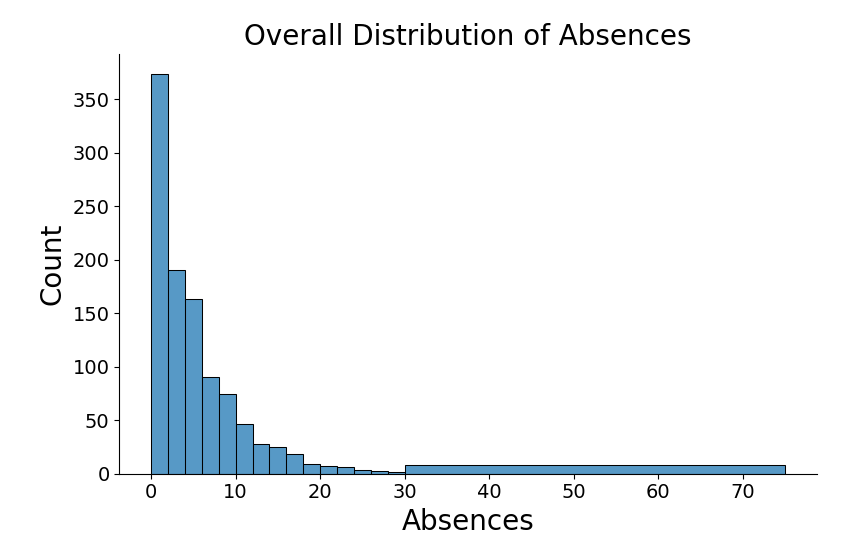
\includegraphics[width = 0.8\textwidth]{fig/Histogram.png}
		\caption{An adjusted histogram with an aggregated bin to emphasize the number of observations with absences greater than 30.}
		\label{histogram}
	\end{figure}
	
	\paragraph{} Many of the binary predictor variables exhibit some class imbalance. For example, over 91\% of all observations replied that they have a desire to pursue higher education, and over 88\% replied that their parents were cohabitating. In contrast, this means that there are only roughly 8 \% of examples from which to learn about students that do not have a desire to pursue higher education, and so on. 
	
	\subsection{Data Disclaimer and Limitations}
	\paragraph{} We discuss some of the limitations regarding our data before moving on to the analysis. First, given the personal nature of the survey, non-response is a concern that may bias the results of our analyses. During collection of the data, personal identifiers were required by the surveyors to merge the survey results with the student's absence records. Indeed, the data authors stated that the responses from 111 students were removed during pre-processing, as they lacked personal identification \cite{Cortez::2008}. One possible concern if whether there was a systematic pattern to which observations were missing. For example, if students who missed classes more often due to poor family relationships, and were also unwilling to identify themselves for the same reason, then any resulting models will have underestimated this effect. Unfortunately without the missing data, it is hard to perform any analysis to assess this, so we will have to assume that our data is sufficiently representative of a random sample. Furthermore, it is possible that students were unwilling to disclose information truthfully. For example, students in a romantic relationship may not be willing to disclose this fact, and it is unclear whether or not students were given an option for non-response. Nonetheless, we believe that there are useful conclusions to be drawn from the data at hand by assuming that it arises from a random sample, and continue with the standard analyses. 
	
	\section{Exploratory Analysis}
	
	\paragraph{} Without assuming any explicit probabilistic models for the data, we can first perform some exploratory analysis of the relationships between the predictor and response variables. To begin, we can examine the effects of each binary predictor on the distribution of absences. Some highlighting facts are presented here, while complete tables are available in the appendix. We refer to students with more than 20 absences as ``highly absent".  
	\begin{itemize}
		\item Of the 23 students with more than 20 absences (highly absent):
		\begin{itemize}
			\item Just 7, or $\approx 30\%$ were male, in comparison to $\approx 43\%$ overall.
			\item 22 out of 23, or $\approx 96\%$ had internet at home, compared to $\approx 79\%$ overall.
			\item 16 out of 23, or $\approx 70\%$ were in romantic relationships, compared to $\approx 36\%$ overall.
		\end{itemize}
		\item The mean number of absences for students with parents cohabiting is $\approx 4.18$ and the proportion of perfect attendance is $35.48\%$. The same statistics are $\approx 6.39$ and $30.58\%$ for separated parents. 
		\item Students without internet at home have a mean absence of $\approx 3.34$, while students with internet have a mean absence of $\approx 4.72$. The proportion of perfect attendance is similar ($1.4\%$ difference), indicating that the mean absences of students with internet is likely carried by the few outliers with $>20$ absences, as explored in the first point. 
	\end{itemize}
	
	\paragraph{}There are some very interesting deviations from the overall data when restricting our view to highly absent students. In particular, there is a much larger proportion of students in romantic relationships who are also highly absent, when compared to the overall population. Also, almost every student who was highly absent also had internet access at home. An important factor to note is that these proportions are expressed over the same 23 individuals, and the causality is not necessarily clear. In other words, it could be that internet access is a stronger cause for absenteeism, but that internet access also suggests a higher rate of romantic relations. Nonetheless, the increase on this subset is most clear over the proportion of students in relationships. We visualize this in a split histogram in Figure \ref{splithistogram}, where each bin is split depending on the predictor. It is clear that the proportion of students in romantic relationships increase with the number of absences, and this is not restricted to just highly absent individuals. 
	
	\begin{figure}[h!]
		\centering
		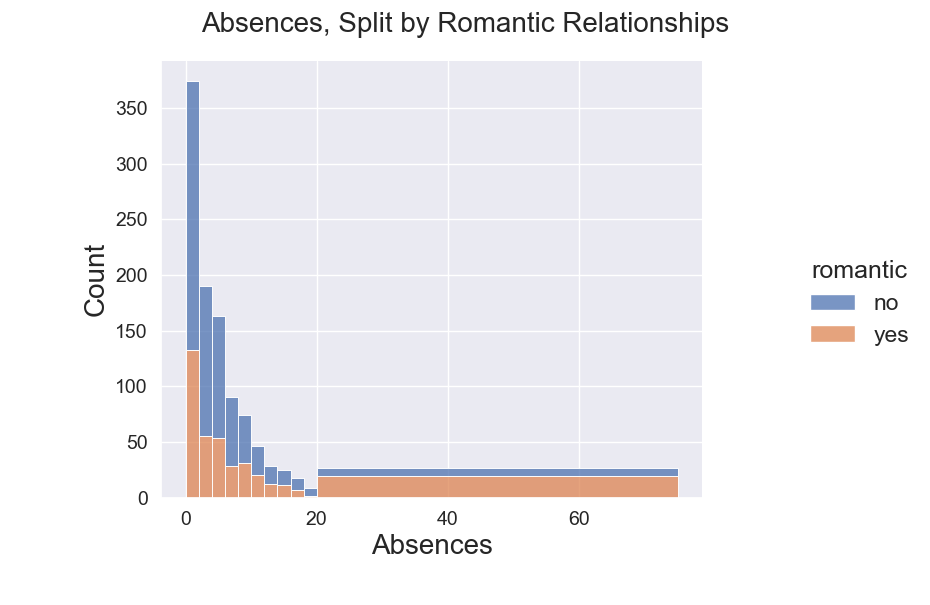
\includegraphics[width = \textwidth]{fig/Hist_Split.png}
		\caption{Histogram in the style of Figure \ref{histogram}, where bins are split depending on whether students are reported to be in a romantic relationship.}
		\label{splithistogram}
	\end{figure}
	
	\paragraph{} We also examine relationships between the remaining covariates and absences. Again, a full table from which the following highlights are obtained from is available in the appendix. 
	
	\begin{itemize}
		\item For the previously defined highly absent students, the mean response to ``\textit{How much alcohol do you consume?}" is $1.70$, compared to $1.49$ overall. 
		\item For students who responded 5 to the family relationship question (i.e., the student perceive the best possible relationship with their family), the mean absences are $3.98$, while those who responded 1 had a mean absence of $5.47$. 
		\item There are 70 students who are 19 and older, while secondary school is typically completed at age 18 in Portugal. Of these students, the mean absences are 7.04, compared to the overall mean of 4.43. 
		\begin{itemize}
			\item An interesting note to make is that for students over 19, the mean alcohol response is $1.79$, and the proportion of those in romantic relationships is $50\%$ (compared to $\approx 36\%$ overall). Both of these factors would already suggest higher absence counts, according to the analysis above. 
		\end{itemize}
	\end{itemize}
	
	\paragraph{} There is also some insight to be gained from examining how these variables relate to whether students will exhibit perfect attendance. This is summarized in Figure \ref{famrel}, which clearly displays that students with poor perceived family relationships are less likely to have perfect attendance over the year. 
	
	\begin{figure}[h!]
	\centering
	\includegraphics[width = \textwidth]{fig/famrel.png}
	\caption{Bar plot of the Likert-scaled response for family relationship. Larger values indicate a better perceived relationship. The orange segment of each bar represents the proportion of individuals who logged perfect attendance.}
	\label{famrel}
	\end{figure}
	
	\section{Regression Analysis}
	\paragraph{} We first introduce some notation to help formulate the models in this section. For $i=1, 2, \dots, n = 1044$, let $Y_i$ be the integer valued response variable and $X_i$ be a d-dimensional vector of predictor variables. For $X_{ij}$, binary variables are coded as $\{0,1\}$ where $X_{ij} = 1$ if it is the reference class. The age and Likert-scale variables are considered to be continuous for the sake of our modeling. We believe this is a reasonable choice as both these variables have ordinal traits and the increments are roughly equal. We first check for co-linearity between the predictor variables to ensure numeric stability and that none of the predictors carry the same information. We observe only mild correlations across the predictors, and choose not to remove any variables for our model. The correlation heat-map is given in Figure \ref{corr}.
	
	\begin{figure}[h!]
		\centering
		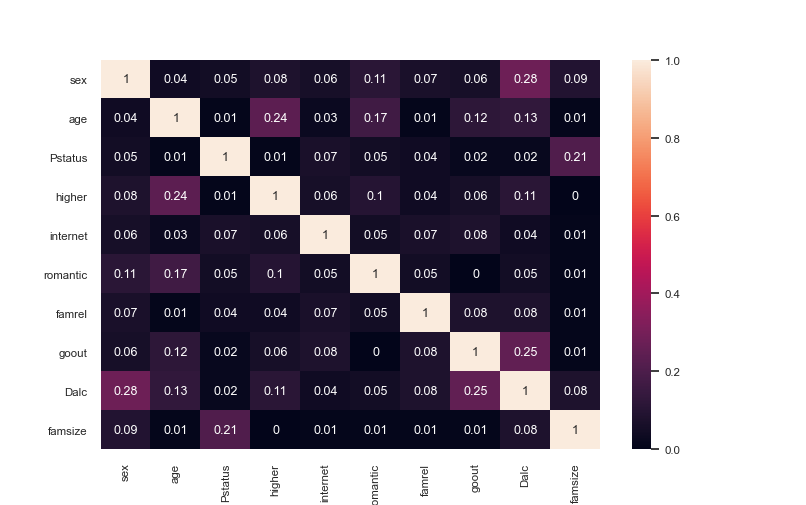
\includegraphics[width = \textwidth]{fig/Correlation.png}
		\caption{Correlation matrix of the predictor variables.}
		\label{corr}
	\end{figure}
	
	\subsection{Poisson Regression}
	\paragraph{} For our confirmatory analysis, we first attempt to fit a Poisson generalized linear model (GLM) to the data. The Poisson GLM is the simplest regression model that respects the integer constraint on our data, and is defined as follows. Let $\beta$ be a d- dimensional vector and $\beta_0$ a scalar, then suppose that
	\begin{gather*}
	Y_i|X_i \sim \text{Poisson}(\mu_i) \\
	\mu_i = \exp(\beta_0 + X_i\beta) \\
	E[Y_i|X_i] = \mu_i = Var[Y_i|X_i]
	\end{gather*} 
	\paragraph{} The optimal model is selected using backwards selection with the BIC penalized log-likelihood, which is found to have 7 predictors including the constant. The entire maximum likelihood fit can be found in the appendix. We provide a Pearson's residual plot by predicting the response by the corresponding mean under the model to assess the fit of the model in Figure \ref{resid}. 
	
	\paragraph{}Since the Poisson model posits that $SD[Y_i] = \sqrt{\mu_i}$, it tends to underestimate the variance of the model here. To see this, note that the mean of the sample is $\bar{Y} \approx 4.43$, yet we have at least 23 cases of $Y > 20$, which is more than 7 standard deviations away under the Poisson model. Furthermore, recall that for a Poisson random variables, we have that:
	$$
	P(Y_i = 0 | X_i) = \exp(-\mu_i) = \exp(-\beta_0 - X_i\beta)
	$$
	%
	\paragraph{} We compute this probability under the fitted model for all observations and obtain that the mean of these probabilities is $25.27\%$. In other words, the model suggests that the students who exhibited perfect attendance should do so with $25.27\%$ probability, given their profiles, on average. Since $35.48\%$ of students exhibit perfect attendance in the data, this suggests that the model is not adequately capturing this portion of students. Furthermore, the model predicts this probability to be just $26.12\%$ on average even amongst the subset of students that have been recorded with perfect attendance.
	
	\subsection{Negative Binomial Regression}
	
	\paragraph{} To remedy the variance underestimation issue, the negative binomial (NegBin) GLM is a natural choice. The NegBin is another model that respects the integer constraints of the response, but includes an additional parameter $\alpha$ to provide a more expressive measure of variance. The model under the $\mu$, $\alpha$ parameterization is then:
	\begin{gather*}
	Y_i|X_i \sim \text{NegBin}(\mu_i, \alpha) \quad \alpha > 0\\ 
	\mu_i = \exp(\beta_0 + X_i\beta) \\
	E[Y_i|X_i] = \mu_i \quad Var[Y_i|X_i] = \mu + \mu^2\alpha
	\end{gather*}
	%
	\paragraph{} Details about this reparametrization compared to the standard negative binomial can be found in the appendix. Note that the response function need not be the same as the Poisson, but this is typically the default choice and is the implementation in most software packages. $\alpha$ is taken to be a constant value over all observations, which is also fitted simultaneously via maximum likelihood. Again, the optimal NegBin model is selected via backwards selection with the BIC penalized log-likelihood, but only 4 predictors were selected here. Interestingly, the NegBin backward selection did not select the constant nor the romantic relationships predictor to include in the model. The full maximum likelihood fit is available in Table \ref{MLE}. The practical advantage over the Poisson model is in the flexible variance term. Whenever the data is over-dispersed under a Poisson GLM, the NegBin GLM is able to capture this by fitting a larger value of $\alpha$. Although the predictions $\mu_i$ are very similar in both models for our data, the increased variance predicted by the NegBin model provides a much more reasonable residual plot with values closer to $\pm 2$ (Figure \ref{resid}). In practice, although the prediction is not necessarily improved, the NegBin GLM is rightfully conservative about its predictions, while the Poisson GLM severely underestimates the uncertainty. 
	
	\begin{figure}[h!]
	\centering
	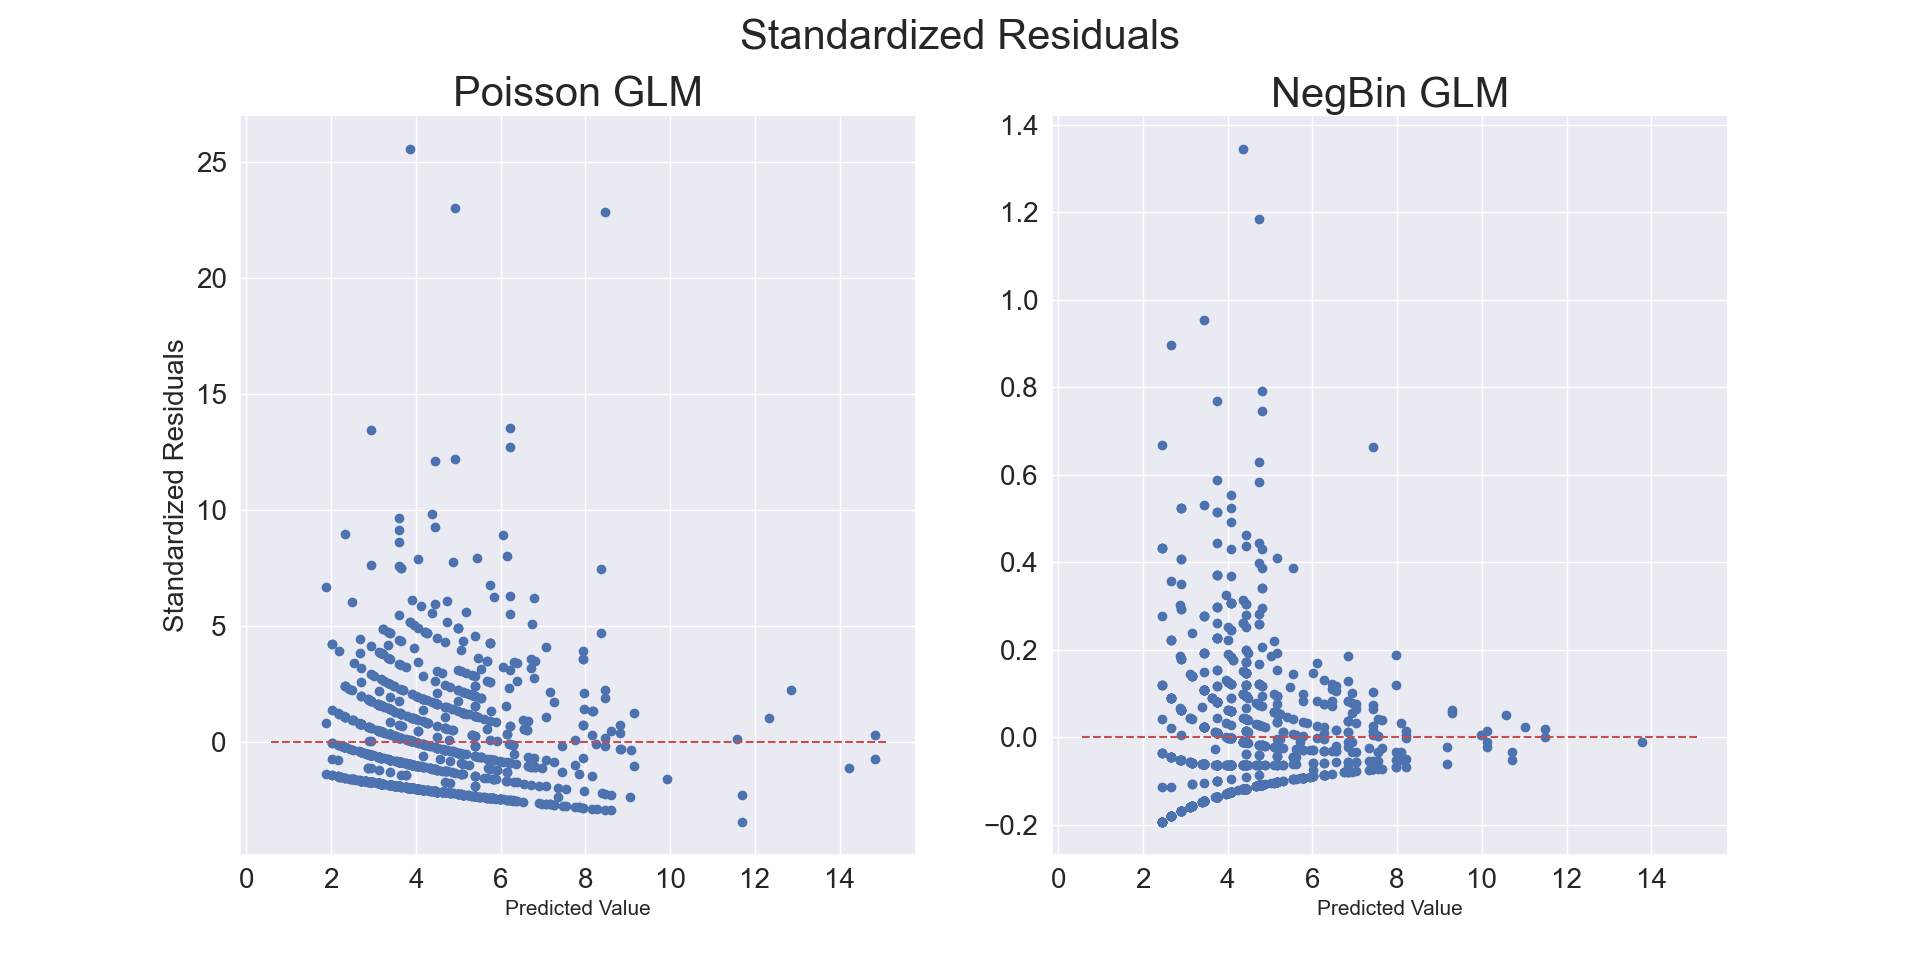
\includegraphics[width = \textwidth]{fig/resid.png}
	\caption{Pearson's residuals (prediction residuals standardized by the predicted standard error) for the Poisson and NegBin GLMs.}
	\label{resid}
	\end{figure}

	\paragraph{} Under the reparametrized negative binomial, the probability of perfect attendance is:
	$$
	P(Y_i = 0 | X_i) = \left(\frac{\alpha^{-1}}{\mu + \alpha^{-1}}\right)^{\alpha^{-1}}  = (1 + \alpha \mu)^{-\alpha^{-1}} = (1 + \alpha \exp(\beta_0 + X\beta))^{-\alpha^{-1}}
	$$
	%
	We compute the mean of this probability to be $29.27\%$ over all samples, and $29.72\%$ over the subset of students with perfect attendance. This is an improvement over the Poisson model, but is still underestimating the proportion of students with perfect attendance at $35.48\%$. 
	
	\subsection{Zero-Inflated Regression Models}
	\paragraph{} To remedy the issue of an excess amount of $0$ responses in the data in comparison to our models, we can turn to zero-inflated modeling \cite{Hall::2004}. The idea is to replace the distributions in the count models above with a simple mixture model, with a point mass at $0$. Suppose the non-inflated distribution of a random variable $Y$ has probability mass function $P(y)$. Then, the probability mass function of the zero-inflated distribution $Y_0$ is:
	$$
	P(y) = \begin{cases}
	p + (1-p)P(y) & y = 0 \\
	(1 - p)P(y) & y > 0
	\end{cases}
	$$
	%
	for any integer $y$, and where $0<p<1$ represents the mixture probability. We have the following facts:
	$$
	E[Y_0] = (1-p)E[Y] \quad Var[Y_0] = (1-p)(Var[Y] + pE[Y]^2)
	$$
	%
	the proof can be found in the appendix. By using a zero-inflated distribution in place of the Poisson and NegBin distributions in the models above, we can hope to better capture the abundance of students with perfect attendance. The interpretation is that with probability $p$, the students will have perfect attendance with certainty. With probability $1-p$, the number of absences will follow whichever base model is specified, as in Section 4. The regular base model is recovered by setting $p=0$ systematically. 
	
	\paragraph{} The specification of zero-inflated models does induce additional complexity in our model. Firstly, $p$ is another parameter to estimate. Furthermore, Figure \ref{famrel} clearly suggests that the probability of perfect attendance, and hence $p$, should also be a function of the predictors. This leads to the usual formulation of zero-inflated models, in which a logistic regression model is fit concurrently to estimate $p$ for each individual. The predictors included in this logistic model can be, but is not necessarily, the predictors included in the main model. Hence, model selection is doubly important in zero-inflated models. Unfortunately, our experiments showed that the zero-inflated models were not able to be fit due to convergence issues when all predictors were included for both the main and logistic model, and thus the backward selection algorithm is not available. However, we found that the forward search algorithm for model selection was still feasible, and thus we select our optimal model using it instead. 
	\section{Zero-inflated Negative Binomial} 
	
	\paragraph{} Given that we have demonstrated that the Poisson regression is inadequate to capture the variance in our dataset, we proceed by considering only the zero-inflated negative binomial model (ZINB). We do provide a model selection and fit for the zero-inflated Poisson in the appendix. Fitting algorithms for ZINB are widely available in many open source statistical software libraries. The forward selection algorithm in this case begins with no predictors for the main and logistic model. However, since at least one predictor must be specified in the main model in order to perform the ZINB fit, on the first iteration we first perform the main model forward selection assuming a constant-only logistic model. Then, the constant only model is used as the main model in the logistic step. This continues until at least one main predictor has been selected, at which point it proceeds as the usual forward selection algorithm iterating over both models simultaneously. Note that each predictor in both models count towards the model complexity that is penalized by AIC or BIC, so ZINB does not strictly outperform the usual NegBin under these objectives. We can formulate this model as follows, where $\gamma_0$ is a scalar and $\gamma$ a $d'$-dimensional vector:
	\begin{gather*}
	Y_i|X_i \sim \begin{cases}
	0 & \text{With probability } p_i \\
	\text{NegBin}(\mu_i, \alpha)  & \text{With probability } 1-p_i
	\end{cases} \quad \alpha > 0
	\\
	\mu_i = \exp(\beta_0 + X_i\beta) \quad p_i = (1 + \exp(\gamma_0 + X_i\gamma))^{-1}  \\  
	E[Y_i|X_i] = (1-p_i)\mu_i \quad Var[Y_i|X_i] = (1-p_i)(\mu + \mu^2\alpha + p_i\mu^2)
	\end{gather*}
	
	\paragraph{} We found that the optimal ZINB under the forward selection algorithm using the BIC penalized log-likelihood included 5 main predictors, which consisted of all predictors included in the usual NegBin model above, as well as the romantic relationships predictor. Only one logistic predictor was selected, corresponding to how often the student goes out with friends. Neither model included the constant term. The residual plot (Figure \ref{ZINBresid}) has deteriorated compared to the standard NegBin model, with many individuals exhibiting standardized residuals of 2 or greater.

	\begin{figure}[h!]
	\centering
	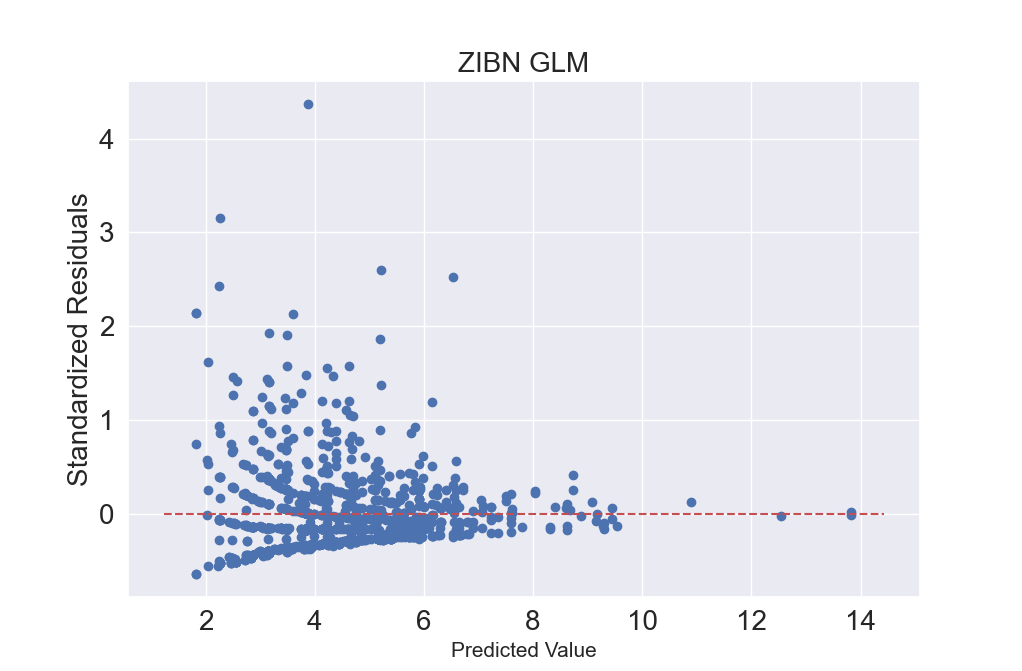
\includegraphics[width = \textwidth]{fig/ZIBNresid.png}
	\caption{Pearson's residuals for the ZINB model.}
	\label{ZINBresid}
	\end{figure}

	\paragraph{} Recall that the probability of perfect attendance under the ZIBN model is now
	$$
	P(Y_i = 0 | X_i) = p_i + (1-p_i)(1 + \alpha \exp(\beta_0 + X\beta))^{-\alpha^{-1}}
	$$
	%
	We compute the mean of this probability to be $34.96\%$, which is very close to the true proportion of students with perfect attendance, and a dramatic improvement over the base models. This result is not surprising, given the resources that we have allocated towards modeling the phenomenon of perfect attendance. 
	
	\section{Final Model Comparison, Selection}
	
	\paragraph{} Having fit three distinct regression models to our data, the interest now lies in selecting the final most appropriate one. Qualitatively, the base Poisson GLM should not be considered, as it dramatically underestimates the variance of the response. Any prediction or inference made with the Poisson would carry with it a foolish confidence. The real model selection question boils down to whether the zero-inflated model was necessary to model the data with a NegBin GLM.
	
	\paragraph{} It is clear that the ZINB model is better suited to correctly model students with perfect attendance, but it does so at the cost of being less computationally flexible and with a more troublesome deviation plot. It is also possible that the forward selection hindered its performance, or that the theoretically best ZIBN model is not even computationally achievable given the precision of our systems. Regardless, in practice and within the scope of this report, the optimal model selected should be viewed as such. The base NegBin GLM provides a pleasing residual plot, and captures perfect attendance better than its Poisson counterpart, but still systematically underestimates the prevalence of this phenomenon. 
	
	\paragraph{} To make a final decision, we turn to quantitative criterion to assess our two competing models. The two models are both fit using maximum likelihood techniques, and the base NegBin model is nested within the ZINB model. Hence, the likelihood ratio test is available. Denote the respective log-likelihoods by $\ell_{NB}(\theta)$ and $\ell_{ZINB}(\theta)$. Since the NegBin model has $5$ estimated parameters and the ZINB has $7$, we have that
	$$
	D = 2(\ell_{ZINB}(\theta) - \ell_{NB}(\theta)) \to \chi_{2}^2
	$$
	%
	where $D$ is the likelihood ratio test statistic. We compute $D = 133.28$ for our test, and since $P(\chi_{2}^2 > 5.98) = 0.95$, and $D >>> 5.98$, we prefer the ZINB test significantly according to the likelihood ratio test. We also compute their BIC-penalized likelihoods in Table \ref{BIC}, which for completeness also includes the Poisson GLM.
	\begin{table}[h!]
		\centering
		\begin{tabular}{|l|l|l|}
			\hline
			Model & $\#$ Parameters & BIC-objective \\
			\hline 
			ZINB & 7 & \textbf{-2585.31}\\
			NegBin & 5 & -2641.99\\
			Poisson & 7 & -4385.53 \\
			\hline
		\end{tabular}
		\caption{BIC-objectives ($\ell(\theta) - \text{BIC}(\theta)$) for all analyzed models. Larger values suggest a better model.}
		\label{BIC}
	\end{table}

	Since the BIC objective is based heavily on the likelihood, it comes as no surprise that it produces a similar result to the likelihood ratio test. However, it should be noted that the gap between the NegBin model and the ZINB model does close somewhat under this objective, as the ZINB model is slightly more complex. Both are significant improvements over the Poisson model as expected. We believe it is valuable to display the maximum likelihood fits of both models in Table \ref{MLE}, as each are applicable for this data depending on the analyst's aim. 
	\begin{table}[h!]
		\centering
		\begin{tabular}{|l|l|l|}
			\hline
			Predictor/Parameter & NegBin Fit & ZINB Fit \\
			\hline 
			Age & 0.08 (0.01) & 0.10 (0.01)\\
			Parents Cohabitate? & -0.52 (0.13) & -0.44 (0.09) \\
			Internet at Home? & 0.34 (0.11) & 0.33 (0.08) \\
			Alcohol Consumption& 0.15 (0.05) & 0.11 (0.3) \\
			Romantic Relationship?& Not Included & 0.20 (0.07) \\
			$\alpha$ & 1.70 (0.10) & 0.53 (0.05) \\
			Go out with friends (ZINB Logistic) & Not Included & -0.28 (0.03) \\
			\hline
		\end{tabular}
		\caption{The full maximum likelihood fit, with standard errors, to the optimal NegBin and ZINB models.}
		\label{MLE}
	\end{table}
	\section{Discussion}
	
	\paragraph{} The above quantitative decision process does not imply that either model is absolutely superior to the other. Although the ZINB fit is only two extra degrees of freedom in terms of information complexity, its practical complexity is far greater than the base NegBin. Not only are there significant convergence issues with computation, but the model is much more difficult to interpret. In practice, it is unclear whether or not the advantages of ZINB can also be realized by fitting a separate logistic regression on the event of perfect attendance, instead of considering it implicitly in a complicated ZINB model. If one model is explicitly desired for the entire data at hand, then ZINB provides a clear option for such a task. However, if the analyst is not interested in the cases of perfect attendance, but merely the conservative and accurate prediction of absence counts, the residual plot associated with the NegBin model indicates that it is a strong contender. We note that as seen in Table \ref{MLE}, the estimates provided are similar across a number of predictors. It is also clear judging by the residual shapes in Figures \ref{resid} and \ref{ZINBresid} that the unstandardized residuals follow a similar pattern.  However, the difference in $\alpha$ is significant, and causes the ZINB to underestimate the variance in comparison to the NegBin, and is the cause of the larger standardized residuals. We believe that this is due to the variance corresponding to the inflated zero values being explained by the logistic component. Another interesting observation is that the base NegBin does not consider the presence of romantic relationships to be a significant predictor of absences, while the exploratory analysis as well as the ZINB model would suggest otherwise.
	\paragraph{} Although the zero-inflated Poisson was not included in the report for brevity, the experiments conducted involving it were more computationally stable, and the backwards search algorithm was compatible. We suspect that in cases without overdispersion that the zero-inflated Poisson may make an even stronger case than the ZINB here. 
	
	\section{Conclusion}
	In this report, we examined the effects of various personal factors in the lives of secondary school students in Portugal on their school attendance records. To achieve this, we fit three different regression models, specialized for count data. According to quantitative criterion, it was revealed that the zero-inflated negative binomial was the most adequate for the data at hand. However, we believe that the basic negative binomial model is also a valuable tool for this dataset, and recommend analysis using either tool for this data, and similar education datasets in the future.
	
	\bibliographystyle{unsrt}
	\bibliography{project_bib}
	
	\newpage 
	
	\section*{Appendix}
	
	\subsection*{Complete Exploratory Analysis}
	
	\paragraph{} The code, including this tex file is available at \url{https://github.com/xijohnny/STAT538_Project}. 
	\paragraph{Highly Absent Students} As defined in the main text, highly absent students are the subset of students that exhibit greater than 20 absences over the year. We provide some summary statistics about this group:
	
	\begin{table}[h!]
		\centering
		\begin{tabular}{|l|l|l|}
			\multicolumn{3}{l}{Total Number of Highly Absent: $n = 23$} \\
			\hline
			Predictor & Mean Value (Highly Absent) & Overall Mean \\
			\hline
			Sex & $30.43\%$ & $43.39 \%$ \\
			Age & 17.35 & 16.73 \\
			Cohabitate & $78.26\%$ & $88.41\%$ \\
			Higher ed. & $86.96\%$ & $91.47\%$ \\
			Internet & $95.65\%$ & $79.21\%$ \\
			Romantic & $69.56\%$ & $35.53\%$ \\
			Fam. Rel. & 3.96 & 3.94 \\
			Go out & 3.17 & 3.16 \\
			Alc. Cons. & 1.69 & 1.49 \\
			Fam Size & $30.43\%$ & $29.31\%$\\
			\hline
		\end{tabular}
	\caption{Summary of highly absent students.}
	\end{table}

	\paragraph{Full Binary Analysis} We provide the table for mean values of absences for different groups of binary predictors.
	
	\begin{table}[h!]
		\centering
		\begin{tabular}{|l|l|l|}
			\hline
			Attribute & Mean Absences & Proportion of Perf. Attendance \\
			\hline
			Male & 4.34 & $33.99\%$ \\
			Female & 4.51 & $34.69\%$ \\
			\hline
			Romantic (Y) & 5.32 & $34.50\%$ \\
			Romantic (N) & 3.95 & $34.32\%$ \\
			\hline
			Cohabitate (Y) & 4.18 & $34.89\%$ \\
			Cohabitate (N) & 6.39 & $30.58\%$ \\
			\hline
			Internet (Y) & 4.72 & $34.09\%$ \\
			Internet (N) & 3.33 & $35.48\%$ \\
			\hline
			$<3$ children & 4.61 & $34.64\%$ \\
			$\geq 3$ children & 4.36 & $34.28\%$ \\
			\hline
		\end{tabular}
	\caption{Summary of binary sliced responses.}
	\end{table}
	
	\paragraph{In depth on family relationships} The following table provides a complete look at the mean absences and proportion of perfect attendance for various levels of family relationships.
	
	\begin{table}[h!]
		\begin{tabular}{|l|l|l|l|}
			\hline
			Fam. Rel. Level & Mean Absences & Proportion of Perf. Attendance & Num. Responses \\
			\hline
			1 & 5.47 & $30.00\%$ & 30 \\
			2 & 5.38 & $21.27\%$ & 47 \\
			3 & 4.81 & $28.40\%$ & 169 \\
			4 & 4.42 & $35.74\%$ & 512 \\
			5 & 3.97 & $38.11\%$ & 286 \\
			\hline
		\end{tabular}
	\caption{Summary of responses sliced by family relationship.}
	\end{table}

	\subsection*{Poisson Models}
	For the base Poisson regression, backwards selection yielded the following optimal model:
	\begin{table}[h!]
		\centering
		\begin{tabular}{|l|l|}
			\hline
			Predictor/Parameter & Poisson MLE Fit  \\
			\hline 
			Constant & -0.81 (0.20) \\
			Age & 0.14 (0.01)  \\
			Parents Cohabitate? & -0.45 (0.04) \\
			Internet at home?& 0.38 (0.04)  \\
			Romantic Relationship?& 0.18 (0.03)  \\
			Family relationship & -0.08 (0.01) \\ 
			Alcohol Consumption & 0.13 (0.01) \\
			\hline
		\end{tabular}
		\caption{Poisson MLE fit.}
	\end{table}

	The zero-inflated Poisson, also using backwards selection yielded the following optimal model:
	
	\begin{table}[h!]
		\centering
		\begin{tabular}{|l|l|l|}
			\hline
			Predictor/Parameter & Main Fit & Logistic Fit  \\
			\hline 
			Sex & -0.09 (0.03) & N/A \\
			Age & 0.11 (0.01) & -0.06 (0.02)  \\
			Parents Cohabitate? & -0.38 (0.04) & N/A \\
			Higher Education? & -0.12 (0.04) & N/A  \\
			Internet at home?& 0.35 (0.04) & N/A \\
			Romantic Relationship?& 0.17 (0.03) & N/A  \\
			Family relationship & N/A & 0.22 (0.07) \\ 
			Alcohol Consumption & 0.09 (0.02) & N/A \\
			Go out with friends & N/A & -0.17 (0.06)\\
			\hline
		\end{tabular}
		\caption{Zero-inflated Poisson fit, with main model and logistic component. If cell is N/A, then the predictor was not included in the optimal model for that component.}
	\end{table}

	Interestingly, the zero-inflated counterpart to the Poisson actually does not include family relationships as a main component, but does as a inflation/logistic component.
	
	\subsection*{Negative Binomial Reparametrization}
	For a random variable $Y$ with the negative binomial distribution, it is usually parametrized by the parameters $(r,p)$, $r>0$ and $p\in[0,1]$ and the PMF is
	$$
	P_Y(y) = \frac{\Gamma(y+r)}{y!\Gamma(r)}(1-p)^{r}p^{y}
	$$
	%
	its moments are
	$$
	E[Y] = \frac{pr}{1-p} \quad Var[Y] = \frac{pr}{(1-p)^2}
	$$
	%
	however, for the sake of regression modelling, it is convenient to instead reparametrize this distribution in terms of the mean. Hence, by setting $\mu = \frac{pr}{1-p}$ and $\alpha = r^{-1}$, we obtain
	$$
	E[Y] = \mu_i \quad Var[Y] = \mu_i + \alpha\mu_i^2
	$$
	%
	and the PMF becomes
	$$
	P_Y(y) = \frac{y + \alpha^{-1}}{y!\Gamma(\alpha^{-1})}\left(\frac{\alpha^{-1}}{\alpha^{-1} + \mu} \right)^{\alpha^{-1}}\left(\frac{\mu}{\alpha^{-1} + \mu} \right)^y
	$$
	%
	from which we can obtain the following probability under the model by considering $P_Y(0)$:
	$$
	P(Y_i = 0 | X_i) = (1 + \alpha \exp(\beta_0 + X\beta))^{-\alpha^{-1}}
	$$
	\subsection*{Zero-inflated Moments}
	We show the following claim where $Y$ is a base distribution supported on the integers and $Y_0$ is its zero-inflated counterpart.
	$$
	E[Y_0] = (1-p)E[Y] \quad Var[Y_0] = (1-p)(Var[Y] + pE[Y]^2)
	$$
	%
	First, we have that
	\begin{gather*}
		E[Y_0] = \sum_{y=0}^{\infty} yP(Y_0 = y) = \sum_{y=1}^{\infty} yP(Y_0 = y) \\
		= (1-p)\sum_{y=1}^{\infty}yP(Y=y) = (1-p)E[Y]
	\end{gather*}
	In the exact same way, we can conclude that
	\begin{gather*}
		E[Y_0^2] = (1-p)E[Y^2] = (1-p)(E[Y]^2 + Var[Y])
	\end{gather*}
	Since $Var[Y] = E[Y^2] - E[Y]^2$. We also have that
	\begin{gather*}
		Var[Y_0] = E[Y_0^2] - E[Y_0]^2 = (1-p)(E[Y]^2 + Var[Y] - (1-p)E[Y]^2) \\
		= (1-p)[V[Y] + pE[Y]^2]
	\end{gather*}
	This shows the claim. For the ZINB model, the moments are shown in section 5. We also display here the moments of the zero-inflated Poisson model as fit above. 
	$$
	E[Y_i|X_i] = (1-p_i)\mu_i \quad  Var[Y_i|X_i] = (1-p_i)(\mu_i + p\mu_i^2)
	$$
\end{document}
